%%%%%%%%%%%%%%%%%%%%%%%%%%%%%%%%%%%%%%%%%%%%%%%
%   Document Class: article, book, memoir,...
%   Check compatibility with Specific packages
%%%%%%%%%%%%%%%%%%%%%%%%%%%%%%%%%%%%%%%%%%%%%%%

\documentclass[12pt, letterpaper]{memoir}

%%%%%%%%%%%%%%%%%%%%%%%%%%%%%%%%%%%%%%%%%%%%%%%
%           Set common of packages 
%%%%%%%%%%%%%%%%%%%%%%%%%%%%%%%%%%%%%%%%%%%%%%%

\usepackage[margin=2.5cm]{geometry}
%\usepackage[T1]{fontenc}
%\usepackage{lmodern}

\usepackage{graphicx}
\usepackage{booktabs}
\usepackage{multirow}
\usepackage{engord}
\usepackage{soul}
\usepackage{parskip}

%---------------- Language -------------------
\usepackage[UKenglish]{babel}
\usepackage[UKenglish]{isodate}

%-------------- CAPTION settings -------------
\usepackage[skip=2pt,font=footnotesize,justification=centering]{caption}

%------------- Maths environment --------------
%\usepackage{amsmath}
\usepackage{mathtools}

%------------- Special Characters -------------
\usepackage{textcomp}


%%%%%%%%%%%%%%%%%%%%%%%%%%%%%%%%%%%%%%%%%%%%%%%
%     To control spaces in Memoir class
%%%%%%%%%%%%%%%%%%%%%%%%%%%%%%%%%%%%%%%%%%%%%%%

\DisemulatePackage{setspace}
\usepackage{setspace}
%\usepackage{titlesec}

%%%%%%%%%%%%%%%%%%%%%%%%%%%%%%%%%%%%%%%%%%%%%%
%           Colours Settings
%%%%%%%%%%%%%%%%%%%%%%%%%%%%%%%%%%%%%%%%%%%%%%

\usepackage[dvipsnames]{xcolor}
% UN Institutional Colours
\definecolor{UNGreen}{RGB}{148,180,59}
\definecolor{UNRed}{RGB}{166,28,49}
\definecolor{UNGreen2}{RGB}{70,107,63}
\definecolor{UNRed2}{RGB}{118,35,47}
\definecolor{UNGray}{RGB}{86,90,92}
\definecolor{UNGrayLight}{RGB}{177,178,176}
% UN Secondary Colours
\definecolor{UNBlack}{RGB}{0,0,0}
\definecolor{UNGray2}{RGB}{153,153,153}
\definecolor{UNBlue}{RGB}{46,58,160}
\definecolor{UNBlueL}{RGB}{30,111,193}
\definecolor{UNGreenL}{RGB}{55,183,146}
\definecolor{UNYellow}{RGB}{244,183,61}
\definecolor{UNPinkL}{RGB}{242,231,204}
\definecolor{UNRedL}{RGB}{232,83,53}
\definecolor{UNPurple}{RGB}{182,17,127}
% sesquicentennial Colours
\definecolor{UNBlueS}{RGB}{15,98,119}
\definecolor{UNGrayS}{RGB}{87,87,87}



%%%%%%%%%%%%%%%%%%%%%%%%%%%%%%%%%%%%%%%%%%%%%%%%%
%         Chapters and Section Styles
%%%%%%%%%%%%%%%%%%%%%%%%%%%%%%%%%%%%%%%%%%%%%%%%%

%------- Fancy Package: check compatibility ----------
%\usepackage{fancyhdr}

% ----- STYLE OF ABSTRACT  (Check Compatibility) -----
%\renewcommand*\abstractname{Summary}
%\abstractintoc

%------------- Default Memoir Styles -----------------
%\chapterstyle{bianchi}
%\chapterstyle{ger}
%\chapterstyle{madsen}
%\chapterstyle{ell}
%\chapterstyle{veelo}

% ----------- Custom chapter: Red Box Style ----------

\makeatletter
\newlength\dlf@normtxtw
\setlength\dlf@normtxtw{\textwidth}
\def\myhelvetfont{\def\sfdefault{mdput}}
\newsavebox{\feline@chapter}
\newcommand\feline@chapter@marker[1][4cm]{%
\sbox\feline@chapter{%
\resizebox{!}{#1}{\fboxsep=1pt%
\colorbox{UNRed2}{\color{white}\bfseries\UNAncizarSerif\thechapter}%
}}%
\rotatebox{90}{%
\resizebox{%
\heightof{\usebox{\feline@chapter}}+\depthof{\usebox{\feline@chapter}}}%
{!}{\scshape\so\@chapapp}}\quad%
\raisebox{\depthof{\usebox{\feline@chapter}}}{\usebox{\feline@chapter}}%
}
\newcommand\feline@chm[1][4cm]{%
\sbox\feline@chapter{\feline@chapter@marker[#1]}%
\makebox[0pt][l]{% aka \rlap
\makebox[1cm][r]{\usebox\feline@chapter}%
}}
\makechapterstyle{daleif1}{
\renewcommand\chapnamefont{\UNAncizarSerif\Large\scshape\raggedleft\so}
\renewcommand\chaptitlefont{\UNAncizarSerif\huge\bfseries\scshape\color{UNRed2}}
\renewcommand\chapternamenum{}
\renewcommand\printchaptername{}
\renewcommand\printchapternum{\null\hfill\feline@chm[2.5cm]\par}
\renewcommand\afterchapternum{\par\vskip\midchapskip}
\renewcommand\printchaptertitle[1]{\chaptitlefont\raggedleft ##1\par}
}
\makeatother
\chapterstyle{daleif1}


% --------- Custom chapter: Blue Box -----------

\newsavebox{\ChpNumBox}
\makeatletter
\newcommand*{\thickhrulefill}{%
\leavevmode\leaders\hrule height 1\p@ \hfill \kern \z@}
\newcommand*\BuildChpNum[2]{%
\begin{tabular}[t]{@{}c@{}}
\makebox[0pt][c]{#1\strut} \\[.5ex]
\colorbox{UNRed}{%
\rule[-10em]{0pt}{0pt}%
\rule{1ex}{0pt}\color{black}#2\strut
\rule{1ex}{0pt}}%
\end{tabular}}
\makechapterstyle{ColorBox}{%
\renewcommand{\chapnamefont}{\large\scshape}
\renewcommand{\chapnumfont}{\Huge\bfseries}
\renewcommand{\chaptitlefont}{\raggedright\Huge\bfseries}
\setlength{\beforechapskip}{20pt}
\setlength{\midchapskip}{26pt}
\setlength{\afterchapskip}{40pt}
\renewcommand{\printchaptername}{}
\renewcommand{\chapternamenum}{}
\renewcommand{\printchapternum}{%
\sbox{\ChpNumBox}{%
\BuildChpNum{\chapnamefont\@chapapp}%
{\chapnumfont\thechapter}}}
\renewcommand{\printchapternonum}{%
\sbox{\ChpNumBox}{%
\BuildChpNum{\chapnamefont\vphantom{\@chapapp}}%
{\chapnumfont\hphantom{\thechapter}}}}
\renewcommand{\afterchapternum}{}
\renewcommand{\printchaptertitle}[1]{%
\usebox{\ChpNumBox}\hfill
\parbox[t]{\hsize-\wd\ChpNumBox-1em}{%
\vspace{\midchapskip}%
\thickhrulefill\par
\chaptitlefont ##1\par}}%
}
%\chapterstyle{ColorBox}

%%%%%%%%%%%%%%%%%%%%%%%%%%%%%%%%%%%%%%%%%%%%%%
%             Page Styles
%%%%%%%%%%%%%%%%%%%%%%%%%%%%%%%%%%%%%%%%%%%%%%

%---------- Default Memoir page style -----------
% (can be included inside the body)
%\pagestyle{ruled}
%\pagestyle{headings}
%\pagestyle{fancy}
%\makepagestyle{fancy}
%\makepagestyle{plain}
%\makeevenfoot{plain}{\thepage}{}{}
%\makeoddfoot{plain}{}{}{\thepage}
%\makeevenhead{fancy}{}{}{}
%\makeoddhead{fancy}{}{}{}


%---------- Custom Page Style --------------

%Example 1:
%\makeheadrule{headings}{\textwidth}{\normalrulethickness}
%\pagestyle{headings}

%Example 2:
%\addtopsmarks{companion}{}{
%\createmark{chapter}{both}{shownumber}{}{. \space}}
%\pagestyle{companion}


%------------ Memoir Example Customisation-----------

% The following code have been found in Peter Wilsons Memoir manual in chapter 7 (page127)
 
\makepagestyle{YourPagestyleName} % Create a new pagestyle
 
% Following code to edit the pagestyle
\makepsmarks{YourPagestyleName}{%
\nouppercaseheads
 
% This is where we specify what \leftmark and \rightmark contains
\createmark{chapter}{both}{shownumber}{}{\space}
\createmark{section}{right}{shownumber}{}{\space}
% Change "shownumber" to "nonumber" if you don't want
%   the chapter/section number displayed at the header.
 
\createplainmark{toc}{both}{\contentsname}
\createplainmark{lof}{both}{\listfigurename}
\createplainmark{lot}{both}{\listtablename}
\createplainmark{bib}{both}{\bibname}
\createplainmark{index}{both}{\indexname}
\createplainmark{glossary}{both}{\glossaryname}}
% Might want to keep those, see the manual for further information.
 
% The following is where you tweek your header
\makeheadrule{YourPagestyleName}{\textwidth}{\normalrulethickness}
\makeevenhead{YourPagestyleName}{\normalfont\bfseries\thepage}{}{\normalfont Chapter \leftmark }
\makeoddhead{YourPagestyleName}{\normalfont Chapter \rightmark}{}{\normalfont\bfseries\thepage}
 
% Activate your new pagestyle
\pagestyle{YourPagestyleName}



%%%%%%%%%%%%%%%%%%%%%%%%%%%%%%%%%%%%%%%%%%%%%%%%%
%     Numbering in Table of Content (TOC)
%%%%%%%%%%%%%%%%%%%%%%%%%%%%%%%%%%%%%%%%%%%%%%%%%

% ----------------- TOC depth --------------------
% chapters, sections, and subsections are numbered
\maxsecnumdepth{subsection} 
% chapters, sections, and subsections are in the TOC
\maxtocdepth{subsection} 

% Subsubsections are numbered and mark in the TOC
\setsecnumdepth{subsubsection}
\maxsecnumdepth{subsubsection}
\settocdepth{subsubsection}
\maxtocdepth{subsubsection} 

%-------- Sec,SubSec and SubsubSec Colours --------
\setsecheadstyle{\Large\bfseries\color{UNRed2}\UNAncizarSerif\raggedright}
\setsubsecheadstyle{\large\bfseries\color{UNRed2}\UNAncizarSerif\raggedright}
\setsubsubsecheadstyle{\bfseries\color{UNRed2}\UNAncizarSerif\raggedright}


%%%%%%%%%%%%%%%%%%%%%%%%%%%%%%%%%%%%%%%%%%%%%%%%%
%               Bibliography
%%%%%%%%%%%%%%%%%%%%%%%%%%%%%%%%%%%%%%%%%%%%%%%%%
\usepackage{natbib}
\usepackage[colorlinks=true, 
    linkcolor=UNRed2,   % color of internal links
    citecolor=UNGreen2, % color of links to bibliography
    filecolor=UNBlue,   % color of file links
    urlcolor=UNBlue]{hyperref}
% For printing
%\usepackage[colorlinks=true, 
%    linkcolor=UNBlack,          
%    citecolor=UNBlack,        
%    filecolor=UNBlack,  
%    urlcolor=UNBlack]{hyperref}


%%%%%%%%%%%%%%%%%%%%%%%%%%%%%%%%%%%%%%%%%%%%%%%%%%
%              Font Styles
%%%%%%%%%%%%%%%%%%%%%%%%%%%%%%%%%%%%%%%%%%%%%%%%%%

%-------------- Sans Serif font ------------------
%\usepackage{sfmath}
%\renewcommand{\familydefault}{\sfdefault} 

%-------------- Charter BT font ------------------
% To use this it have to be commented
%\usepackage{amssymb}
\usepackage[bitstream-charter]{mathdesign}

%------- UN Official Font: Ancizar family --------
\usepackage{fontspec}
%\usepackage{dsfont}
\setmainfont{AncizarSerif}[
Path = Ancizar/,
Extension       = .otf,
UprightFont     = *-Regular,
BoldFont        = *-Semibold,
ItalicFont      = *-LightItalic,
BoldItalicFont  = *-SemiboldItalic,
%SlantedFont     = *-⟨font name⟩,
%BoldSlantedFont = *-⟨font name⟩,
%SmallCapsFont   = *-⟨font name⟩,
]
\setsansfont{AncizarSerif}[
Path = Ancizar/,
Extension       = .otf,
UprightFont     = *-Regular,
BoldFont        = *-Semibold,
ItalicFont      = *-LightItalic,
BoldItalicFont  = *-SemiboldItalic,
%SlantedFont     = *-⟨font name⟩,
%BoldSlantedFont = *-⟨font name⟩,
%SmallCapsFont   = *-⟨font name⟩,
]

% Define Font callable name
\newfontfamily{\UNAncizarSerif}{AncizarSerif}
[
Path = Ancizar/,
Extension = .otf, 
UprightFont = *-Regular, 
BoldFont= *-Semibold,
ItalicFont      = *-LightItalic,
BoldItalicFont  = *-SemiboldItalic
]
% e.g. {\UNAncizarSerif This text uses the Ancizar Serif font}


%%%%%%%%%%%%%%%%%%%%%%%%%%%%%%%%%%%%%%%%%%%%%%%%
%               Microtype 
%%%%%%%%%%%%%%%%%%%%%%%%%%%%%%%%%%%%%%%%%%%%%%%%

% Using Special package: Microtype 
\usepackage[activate={true,nocompatibility},final,tracking=true,stretch=10,shrink=10]{microtype}

%%%%%%%%%%%%%%%%%%%%%%%%%%%%%%%%%%%%%%%%%%%%%%%
%             Latex Figures
%%%%%%%%%%%%%%%%%%%%%%%%%%%%%%%%%%%%%%%%%%%%%%%
% Graphics with Tikz
\usepackage{tikz}

%%%%%%%%%%%%%%%%%%%%%%%%%%%%%%%%%%%%%%%%%%%%%%%
%           Personal Commands
%%%%%%%%%%%%%%%%%%%%%%%%%%%%%%%%%%%%%%%%%%%%%%%
\newcommand{\ie}{\emph{i.e.}\ }
\newcommand{\eg}{\emph{e.g.}\ }
\newcommand{\etal}{\emph{et al}}
\newcommand{\sub}[1]{$_{\textrm{#1}}$}
\newcommand{\super}[1]{$^{\textrm{#1}}$}
\newcommand{\degC}{$^{\circ}$C}
\newcommand{\wig}{$\sim$}
\newcommand{\ord}[1]{\engordnumber{#1}}
\newcommand{\num}[2]{$#1\,$#2}
\newcommand{\range}[3]{$#1$-$#2\,$#3}
\newcommand{\roughly}[2]{$\sim\!#1\,$#2}
\newcommand{\area}[3]{$#1 \! \times \! #2\,$#3}
\newcommand{\vol}[4]{$#1 \! \times \! #2 \! \times \! #3\,$#4}
\newcommand{\cube}[1]{$#1 \! \times \! #1 \! \times \! #1$}
\newcommand{\figref}[1]{Figure~\ref{#1}}
\newcommand{\eqnref}[1]{Equation~\ref{#1}}
\newcommand{\tableref}[1]{Table~\ref{#1}}
\newcommand{\secref}[1]{Section \ref{#1}}
\newcommand{\XC}{\emph{exchange-correlation}}
\newcommand{\abinit}{\emph{ab initio}}
\newcommand{\Abinit}{\emph{Ab initio}}
\newcommand{\Lonetwo}{L1$_{2}$}
\newcommand{\Dznt}{D0$_{19}$}
\newcommand{\Dtf}{D8$_{5}$}
\newcommand{\Btwo}{B$_{2}$}
\newcommand{\fcc}{\emph{fcc}}
\newcommand{\hcp}{\emph{hcp}}
\newcommand{\bcc}{\emph{bcc}}
\newcommand{\Ang}{{\AA}}
\newcommand{\inverseAng}{{\AA}$^{-1}$}
\renewcommand{\comment}[1]{\textcolor{UNRed}{[COMMENT: #1]}}
\newcommand{\more}{\textcolor{UNRed}{[MORE]}}
\newcommand{\red}[1]{\textcolor{UNRed}{#1}}

% ------- Change this to modify ---------
% ------look of header and footer -------
% (need: fancyhrd package)
%\lhead{}
%\chead{}
%\rhead{}
%\lfoot{}
%\cfoot{\thepage{}}
%\rfoot{}
%\renewcommand{\headrulewidth}{0pt}
%\renewcommand{\footrulewidth}{0pt}



%-%-%-%-%-%-%-%-%-%-%-%-%-%-%-%-%-%-%-%-%-%-%-%-%-%-%-%
%               Beginning of Document
%-%-%-%-%-%-%-%-%-%-%-%-%-%-%-%-%-%-%-%-%-%-%-%-%-%-%-%

\begin{document}

% -------------------- Cover Page ---------------------


% ------------------- Title Page ----------------------

\onehalfspacing

\begin{center}
\includegraphics[width=10em]{Pics/UN_Shield.pdf}

\vspace{0.2in}
{\Large \textit{\color{UNBlueS}Universidad Nacional de Colombia}}
%\includegraphics[width=4in]{Pics/UN_FirmaHorizontal.png}

\vspace{0.8in}

{\Huge \textbf{\color{UNRed2}UN Custom Parameters to use in \LaTeX{} Documents } }

\vspace{0.5in}

{\Large \textbf{\color{UNBlack}Sebastian Rivas Bello}}

%\vfill{}
\vspace{1.2in}
Final project report submitted\\ 
in partial fulfilment for the degree of\\
M.ENG. IN NUCLEAR ENGINEERING
\end{center}

\vfill{}

Date:\today{}     \hfill{} Project supervisor: \\
Word count: 7,999   \hfill{} Dr Alessandro Mottura
\thispagestyle{empty}

% ---------------- Abstract --------------------

%\newpage{}
\chapter*{Abstact}
%\addcontentsline{toc}{chapter}{Abstact}

A summary of the scope and significance of the project, the methodology / techniques used, the results gained / outcomes generated and the conclusions obtained. Abstracts are generally a single paragraph and less than 250 words.

\thispagestyle{empty}



% ---------------- Resumen ---------------------
\clearpage
\chapter*{Resumen}
%\addcontentsline{toc}{chapter}{Resumen}

Un resumen del alcance y la importancia del proyecto, la metodología / técnicas utilizadas, los resultados obtenidos / los resultados generados y las conclusiones obtenidas. Los resúmenes son generalmente de un solo párrafo y menos de 250 palabras.

\thispagestyle{empty}

% --------- Tables: Contents,Table & Figures --------------
\clearpage
\tableofcontents*
%\listoftables          % required if there are tables
%\listoffigures         % required if there are figures
\thispagestyle{empty}


%-%-%-%-%-%-%-%-%-%-%-%-%-%-%-%-%-%-%-%-%-%-%-%-%-%-%-%
%               Beginning of Chapters
%-%-%-%-%-%-%-%-%-%-%-%-%-%-%-%-%-%-%-%-%-%-%-%-%-%-%-%
\clearpage
\pagenumbering{arabic} 
\singlespacing
%\onehalfspacing

%--------------- Introduction ---------------

\chapter{Introduction}
An introduction to the project -- your aims and objectives should go here. You can use bullet points. You probably want to keep this to half-page or so.

\section{First Sec}

{\UNAncizarSerif This text is in AncisarSerif}

\subsection{First Subsec}

{\UNAncizarSerif This text is in AncisarSerif}


\subsubsection{First Subsubsec}


\chapter{Literature review}
This should demonstrate a sound understanding of the current state of knowledge in the field, which should critically assess previous and current work in the public domain, drawing out the major facts, views, trends etc. (not just listing a series of literature / information sources and/or literature/ information abstracts). 

This should then develop into a description of the need for the project and so define the
project aims and how they are to be attained in the methodology and/or experimental work. Literature in \LaTeX{}  is best done using BibTeX. For your individual project you are asked to use the Harvard method for citations -- \LaTeX{} can do it very easily (see above).





\chapter{Methodology}
Description of the methodology and/or experimental methods used to achieve aims of the project in sufficient detail to allow other researchers to repeat your work.





\chapter{Results}
This should be a coherent presentation of the results / outcomes of your work, including your methodology and/or experimental work, such that the key findings i.e. facts, views, trends etc. are readily revealed (this should not be a chronological presentation of what was carried out nor, usually, just the raw data).

\begin{figure}[htbt]
\begin{center}
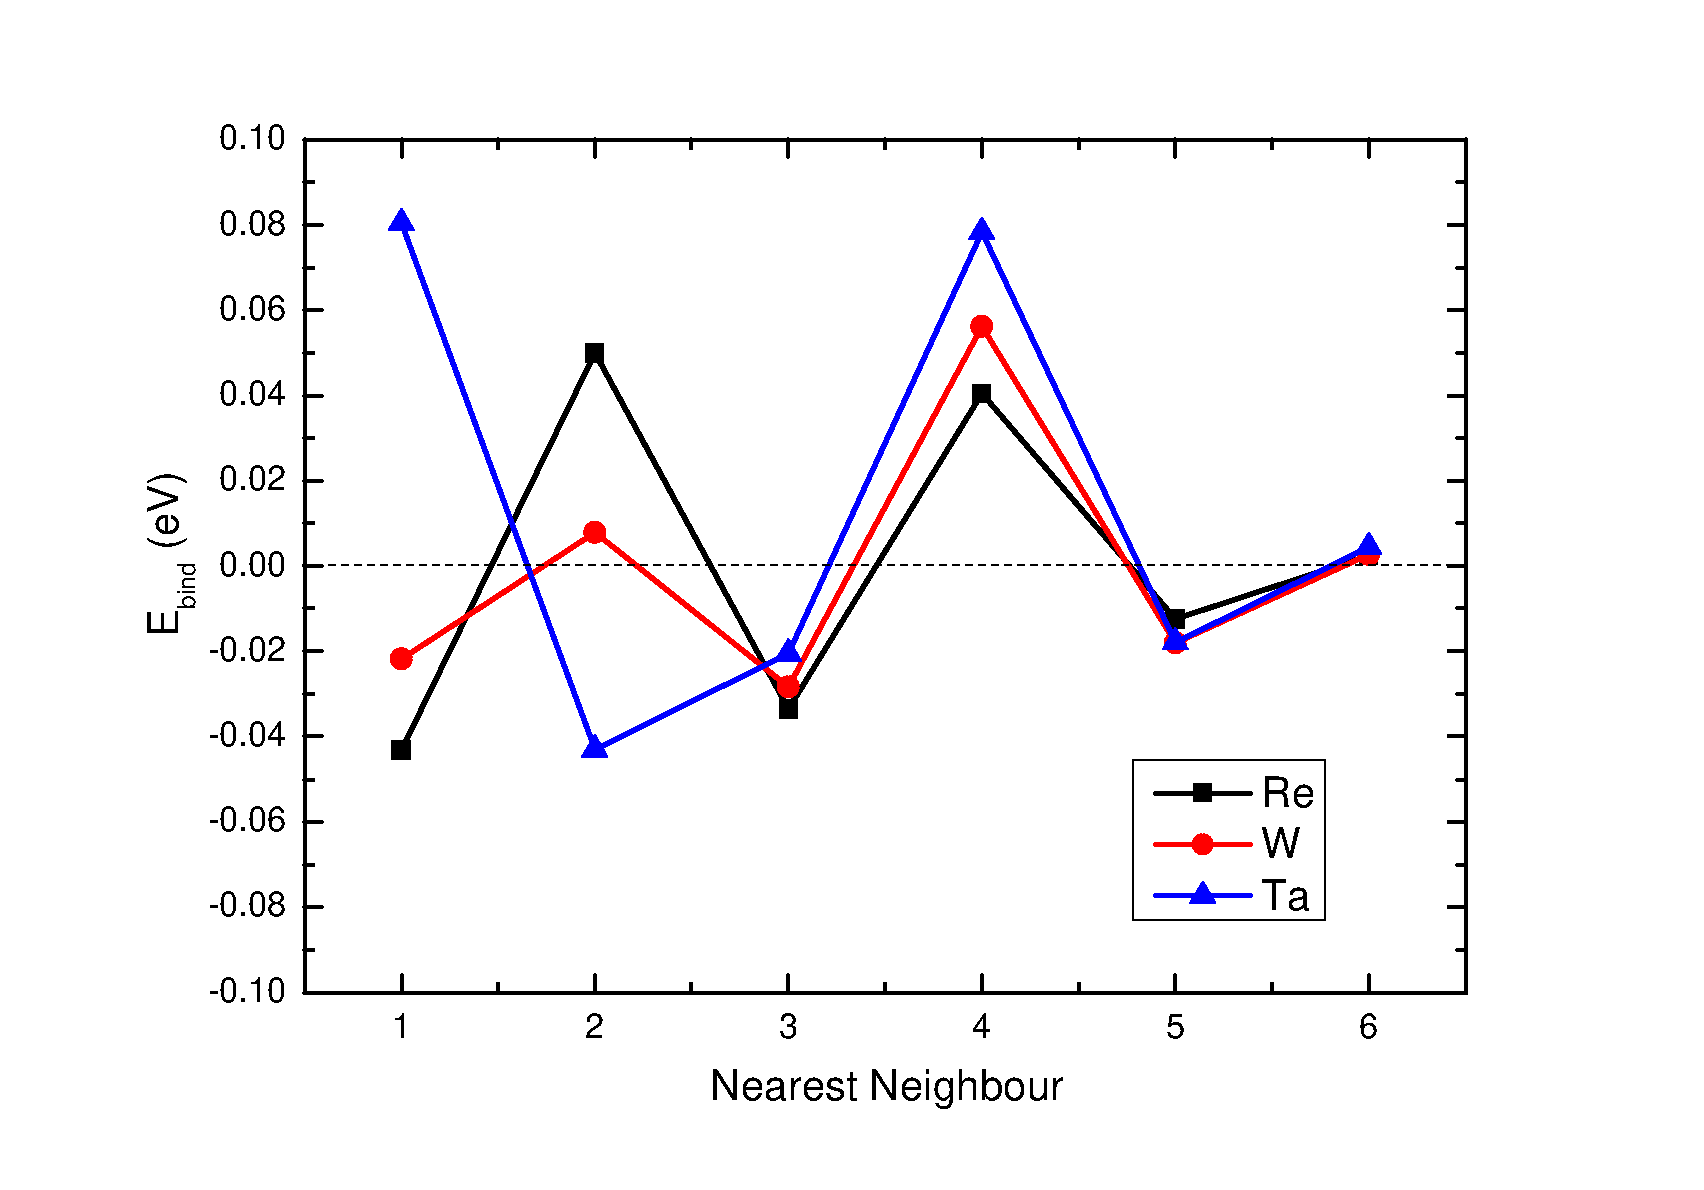
\includegraphics[width=4in]{Pics/examplefig}
\caption{Some example figure}
\label{examplefig}
\end{center}
\end{figure}

A good example of how to insert a figure in \LaTeX{} is shown in \figref{examplefig}. Note that in \LaTeX{} all figures are \emph{floats}. This means they are items that flow all the way to the top of the page.

The kaobook class is based on scrbook, therefore it 
understands all of the options you would normally pass to that class. If 
you have a lot of patience, you can read the guide.\footnote{The guide can be downloaded from 
\url{https://ctan.org/pkg/koma-script?lang=en}.} Actually, the reading 
of such guide is suggested as it is very instructive.

The kaobook class is based on scrbook, therefore it 
understands all of the options you would normally pass to that class. If 
you have a lot of patience, you can read the guide.\footnote{The guide can be downloaded from 
\url{https://ctan.org/pkg/koma-script?lang=en}.} Actually, the reading 
of such guide is suggested as it is very instructive.


\section{Example Section}

 {\bfseries\slshape foo}  {\small \bfseries\textit foo}



\chapter{Discussion}
An analysis of the results of your methodology and/or experimental work, relating the findings back to the assessment of current state of understanding presented in the introduction.


\chapter{Conclusions}
A well-defined summary of the major findings and their interpretation (this should not be further discussion of the results or speculate on areas not assessed in the results and discussion).


%-%-%-%-%-%-%-%-%-%-%-%-%-%-%-%-%-%-%-%-%-%-%-%-%-%-%-%
%                    Appendix
%-%-%-%-%-%-%-%-%-%-%-%-%-%-%-%-%-%-%-%-%-%-%-%-%-%-%-%

\appendix

\chapter{Additional}
Lorem ipsum dolor sit amet, consectetur adipiscing elit, sed do eiusmod tempor incididunt ut labore et dolore magna aliqua. Ut enim ad minim veniam, quis nostrud exercitation ullamco laboris nisi ut aliquip ex ea commodo consequat. Duis aute irure dolor in reprehenderit in voluptate velit esse cillum dolore eu fugiat nulla pariatur. Excepteur sint occaecat cupidatat non proident, sunt in culpa qui officia deserunt mollit anim id est laborum. \citep{hk}


%-%-%-%-%-%-%-%-%-%-%-%-%-%-%-%-%-%-%-%-%-%-%-%-%-%-%-%
%               Bibliography
%-%-%-%-%-%-%-%-%-%-%-%-%-%-%-%-%-%-%-%-%-%-%-%-%-%-%-%


\bibliographystyle{unsrt}
\bibliography{Bibliography/Literature.bib}




\end{document}



